% src/stand_der_technik.tex - Stand der Technik und technologischer Kontext

\subsection{Motion-Capture-Technologien für Live-Performance}

\textbf{Markerbasierte Systeme:}

\raggedright Kommerzielle Motion-Capture-Systeme wie OptiTrack und Vicon verwenden reflektierende Marker und Infrarot-Kameras für hochpräzise Bewegungserfassung. Diese Systeme erreichen Sub-Millimeter-Genauigkeit, erfordern jedoch kontrollierte Umgebungen mit spezieller Beleuchtung und aufwändiger Marker-Platzierung am Performer. Für Live-Performance-Anwendungen stellen die Marker-Anforderungen und Umgebungs-Restriktionen praktische Limitierungen dar \cite{kitagawa2017mocap}.

\textbf{Markerlose Ansätze:}

\raggedright Die Microsoft Kinect-Serie etablierte markerlose Motion-Capture für Consumer-Anwendungen. Die Kinect V1 (2010) nutzte strukturiertes Licht, während die Kinect V2 (2013) Time-of-Flight-Technologie für verbesserte Tiefenerfassung implementierte. Native Kinect-Skelett-Tracking basiert auf Random Forest-Algorithmen, die bei partieller Okklusion und variablen Lichtverhältnissen Limitierungen zeigen \cite{shotton2011real}.

\textbf{Maschinelles Lernen in Pose-Estimation:}

\raggedright OpenPose (2017) von Cao et al. demonstrierte erstmals zuverlässige Echtzeit-Pose-Estimation basierend auf Convolutional Neural Networks \cite{cao2017realtime}. Google's MediaPipe (2019) erweiterte diesen Ansatz durch optimierte Mobile-Implementierung und verbesserte Robustheit bei schwierigen Beleuchtungsbedingungen.

\begin{figure}[htbp]
    \centering
    \adjustbox{max width=0.9\textwidth, max height=0.8\textheight, keepaspectratio}{%
        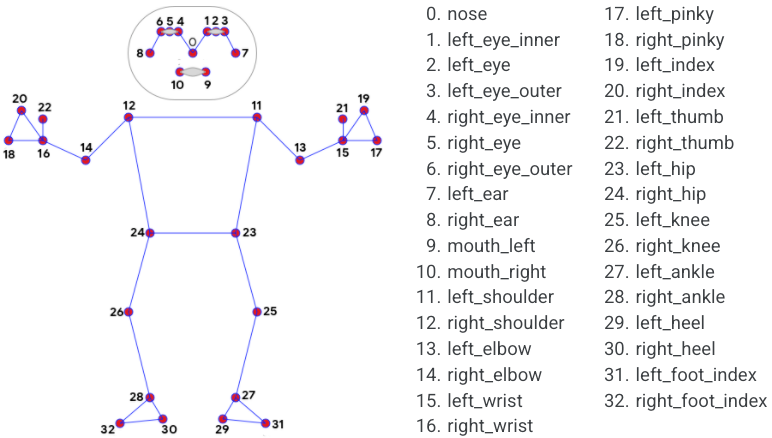
\includegraphics{images/docupictures/mediapipeNODES.png}%
    }
    \caption{MediaPipe Skeleton-Nodes, die die Basis für die Skelett-Visualisierung bilden}
    \label{fig:mediapipe_nodes}
\end{figure}

\textbf{Relevante Erkenntnisse für M.A.S.K.:}
\begin{itemize}
    \item MediaPipe zeigt robustere Performance bei unvollständiger Skelett-Sichtbarkeit
    \item Kombinierte Ansätze können Limitierungen einzelner Sensoren kompensieren
\end{itemize}

\subsection{Interaktive Visualisierungssysteme}

\textbf{TouchDesigner in Performance-Kunst:}

\raggedright TouchDesigner etablierte sich als Standard-Platform für interaktive Medienkunst durch node-basierte visuelle Programmierung und Echtzeit-Rendering-Capabilities. Projekte wie Klaus Obermaier's \glqq Apparition\grqq{} (2004) demonstrierten frühe Anwendungen von Motion-Capture für responsive Bühnenvisualisierung \cite{obermaier2004apparition}.

\textbf{Echtzeit-Rendering-Anforderungen:}

\raggedright Live-Performance erfordert konstante Framerates und minimale Latenz zwischen Eingabe und visueller Ausgabe. Studien zeigen, dass Latenz über 40ms von Performern als störend wahrgenommen wird \cite{flach2004latency}. Dies definiert technische Anforderungen für Motion-Capture-Pipelines in interaktiven Anwendungen.

\subsection{Sensor-Fusion-Ansätze}

\textbf{Kalman-Filter für Motion-Tracking:}

\raggedright Kalman-Filter werden seit den 1960er Jahren für Tracking-Anwendungen eingesetzt und bieten theoretische Grundlagen für wirksame Zustandsschätzung bei verrauschten Sensordaten. Welch und Bishop (2006) dokumentieren Anwendungen für Computer-Vision und Motion-Tracking \cite{welch2006kalman}.

\textbf{Multi-Sensor-Fusion:}

\raggedright Aktuelle Forschung untersucht Kombinationen verschiedener Sensor-Modalitäten für robustere Motion-Capture. Liu et al. (2019) demonstrieren verbesserte Tracking-Stabilität durch Fusion von RGB-, Depth- und IMU-Daten \cite{liu2019multimodal}.

\subsection{Technologische Lücken und M.A.S.K.-Positionierung}

\textbf{Identifizierte Forschungslücken:}

\begin{itemize}
    \item \textbf{Beleuchtungs-Robustheit:} Bestehende Systeme versagen bei intensiver Beamer-Beleuchtung auf Performern
    \item \textbf{Setup-Komplexität:} \raggedright Kommerzielle Systeme erfordern aufwändige Kalibrierung für verschiedene Kamera-Beamer-Konfigurationen
    \item \textbf{Cost-Accessibility:} \raggedright Professionelle Motion-Capture-Systeme überschreiten Budget-Rahmen von Bildungsinstitutionen und Independent-Artists
\end{itemize}

\textbf{M.A.S.K.-Beitrag zur Forschungslandschaft:}

M.A.S.K. adressiert diese Lücken durch:
\begin{itemize}
    \item Infrarot-basierte Tracking-Pipeline für Beleuchtungs-Immunität
    \item Consumer-Hardware-Basis (Kinect V2, Standard-Computer) für Cost-Effectiveness
    \item Parametrische Kalibrierung für schnelle Setup-Anpassungen
    \item Open-Source-Verfügbarkeit für Bildungs- und Forschungsanwendungen
\end{itemize}

\subsection{Verwandte Arbeiten in interaktiver Performance}

\textbf{Akademische Projekte:}

\raggedright Das Interactive Architecture Lab des Bartlett College entwickelte ähnliche Systeme für responsive Rauminstallationen, fokussierte jedoch auf statische Installationen ohne Live-Performance-Anforderungen \cite{achten2011interactive}.

\textbf{Industrielle Anwendungen:}

\raggedright Microsoft's HoloLens und Magic Leap demonstrieren Echtzeit-Hand-Tracking für Augmented Reality, jedoch ohne Integration in Projection-Mapping-Workflows für Performance-Kunst.

\textbf{Differenzierung:}

\raggedright M.A.S.K. unterscheidet sich durch spezifische Fokussierung auf cinematographische Live-Performance unter professionellen Produktionsbedingungen, während bestehende Systeme auf kontrollierte Umgebungen oder Consumer-Anwendungen ausgerichtet sind.